% !TeX program = xelatex
% !TeX encoding = UTF-8
\documentclass[UTF8,12pt,a4paper,fontset=windows]{ctexart}

\usepackage{amsmath,amssymb}
\usepackage{geometry}
\usepackage{graphicx}
\usepackage{booktabs}
\usepackage{array}
\usepackage{float}
\usepackage{placeins}
\usepackage{needspace}
\usepackage{tikz}
\usetikzlibrary{arrows.meta,positioning}
\usepackage[hidelinks]{hyperref}
\geometry{left=2.5cm,right=2.5cm,top=2.2cm,bottom=2.2cm}
\hypersetup{pdftitle={基于 Give Me Some Credit 的信用评分卡分析},pdfauthor={s0Ap224}}
\linespread{1.18}
\setlength{\parskip}{0pt}
\pagestyle{plain}
\ctexset{
  section={format=\Large\bfseries,beforeskip=1.2ex,afterskip=0.8ex},
  subsection={format=\large\bfseries,beforeskip=1.0ex,afterskip=0.6ex},
  paragraph={beforeskip=0pt}
}

\begin{document}
\begin{center}
  {\LARGE\bfseries 基于 Give Me Some Credit 的信用评分卡分析}\\[0.45em]
  {\small 公开作品集版 \quad \href{https://github.com/s0Ap224/credit-risk-scorecard}{s0Ap224 / credit-risk-scorecard}}
\end{center}
\vspace{0.3em}

\section{业务目标与样本划分}
\subsection{明确建模对象}
% !TeX root = ../main.tex

本研究以 Kaggle 原始 Give Me Some Credit 竞赛中的匿名个人借款人信用记录为评分对象，
在历史特征已可取得、未来表现尚未发生的评分时点 $t_0$，利用年龄、收入、负债、
授信使用情况及历史逾期记录等信息，预测该借款人在随后两年内发生
90 天及以上严重逾期或更严重情形的概率。
目标变量为 \texttt{SeriousDlqin2yrs}，取值 1 表示发生目标事件，取值 0 表示未发生，
分别称为坏样本与好样本。评分用于风险排序、预警复核以及后续教学情景下的
风险标记和模拟接受决策；模型概率越高，风险越高，转换后的评分卡则统一采用分数越高、风险越低的方向。

\paragraph{观察窗口、评分时点与表现窗口。}
如图~\ref{fig:time-window} 所示，特征构造与结果观察以 $t_0$ 为界：
\begin{enumerate}
  \setlength{\itemsep}{0.15em}
  \setlength{\parskip}{0pt}
  \item \textbf{观察窗口：}汇总评分时点之前已形成且在 $t_0$ 可获得的个人财务和信用历史，
  构造特征向量 $\boldsymbol{x}_i$（包含年龄、月收入、负债收入比等全部10个特征）。
  \item \textbf{评分时点：}在 $t_0$ 基于已有信息计算个体风险；行号仅用于追踪记录，
  不进入预测特征，未来表现信息（SeriousDlqin2yrs）不参与特征构造。
  \item \textbf{表现窗口：}按照竞赛任务设定，在 $t_0$ 后两年内观察是否发生目标事件，
  待窗口结束、标签成熟后评价预测结果。
\end{enumerate}

令 $Y_i$ 表示第 $i$ 条记录对应借款人在两年表现窗口内的目标事件，则
\begin{equation}
  Y_i=
  \begin{cases}
    1, & \text{两年表现窗口内发生严重逾期或更严重情形},\\
    0, & \text{该窗口内未发生上述目标事件},
  \end{cases}
  \qquad
  p_i=P\!\left(Y_i=1\mid\boldsymbol{x}_i\right).
  \label{eq:prediction-target}
\end{equation}

\begin{figure}[htbp]
  \centering
  \begin{tikzpicture}[
    box/.style={draw=blue!55!black,fill=blue!3,rounded corners=2pt,
      minimum height=2.05cm,text width=4.05cm,align=center,inner sep=6pt,
      font=\small},
    flow/.style={-{Latex[length=2.2mm]},thick,draw=blue!65!black}
  ]
    \node[box] (history) at (-5.15,0) {
      \textbf{历史特征／观察窗口}\\[4pt]
      财务状况、授信使用\\
      与历史逾期信息\\[3pt]
      $\boldsymbol{x}_i$：评分时已可取得
    };
    \node[box] (scoring) at (0,0) {
      \textbf{预测时点 $t_0$}\\[4pt]
      输入已有特征\\
      计算风险概率 $p_i$\\[3pt]
      未来目标事件尚未观察
    };
    \node[box] (outcome) at (5.15,0) {
      \textbf{未来两年／表现窗口}\\[4pt]
      90 天及以上严重逾期\\
      或更严重情形\\[3pt]
      窗口成熟后确定标签 $Y_i$
    };
    \draw[flow] (history.east) -- (scoring.west);
    \draw[flow] (scoring.east) -- (outcome.west);
  \end{tikzpicture}
  \caption{历史特征、预测时点与表现窗口的关系（示意图不按时长比例绘制）}
  \label{fig:time-window}
\end{figure}

\paragraph{时间口径与应用范围。}
上述两年表现窗口依据竞赛任务及本次作业设定。
公开文件未提供逐户评分日期，无法据此还原各人的观察窗口起止日期；
各历史变量的统计口径以数据字典为准。


\subsection{固定样本划分}
\label{sec:sample-split}
% !TeX root = ../main.tex
\newcommand{\SplitSeed}{20261103}
\newcommand{\LabeledDuplicateExcess}{609}
\newcommand{\FeatureDuplicateGroups}{354}
\newcommand{\FeatureDuplicateRows}{1,000}
\newcommand{\CrossSplitFeatureGroups}{246}


以 \texttt{SeriousDlqin2yrs} 为分层标签，固定随机种子为 \SplitSeed，
将全部 150,000 条记录按 $60\%/20\%/20\%$ 划分。
先分出 $60\%$ 的训练集，再将剩余 $40\%$ 等分为验证集和测试集；
两次均使用同一随机种子并按标签分层。
各子集规模与坏样本率见表~\ref{tab:sample-split}。
分层使各部分的事件比例接近总体的 $6.684\%$。

\begin{table}[htbp]
  \centering
  \caption{固定分层随机划分的样本构成（坏样本为正类）}
  \label{tab:sample-split}
  \small
  \begin{tabular}{lrrrrr}
\toprule
子集 & 样本数 & 好样本数 & 坏样本数 & 坏样本率 & 样本占比 \\
\midrule
训练集 & 90,000 & 83,984 & 6,016 & 6.684\% & 60\% \\
验证集 & 30,000 & 27,995 & 2,005 & 6.683\% & 20\% \\
测试集 & 30,000 & 27,995 & 2,005 & 6.683\% & 20\% \\
\midrule
合计 & 150,000 & 139,974 & 10,026 & 6.684\% & 100\% \\
\bottomrule
\end{tabular}

\end{table}

\paragraph{重复与同源记录核查}
原始行号唯一，但仅作为追踪键。
排除行号后，按十个特征和标签检查完全重复记录，发现
\LabeledDuplicateExcess{} 条相对于各组首条的重复行；
仅按十个特征（含缺失位置）匹配，有 \FeatureDuplicateGroups{} 组、
共 \FeatureDuplicateRows{} 条记录，其中 \CrossSplitFeatureGroups{} 组分布在多个子集。
因缺少客户主键（名称或者用户id等唯一编码信息）和逐户日期，无法确认这些记录是否来自同一借款人，
故本次保留原始全部行，按指定比例进行记录层面的分层留出，即以每行为划分单位，
在好、坏样本中分别按比例随机划分训练、验证和测试集，不要求同特征记录进入同一集合。


\paragraph{各部分用途}
训练集用于估计清洗参数、分箱切点、档位合并规则、WOE、IV 以及模型系数；
验证集用于比较和选择模型方案、概率校准方案与决策阈值；
待数据处理规则、模型及阈值全部冻结后，测试集仅承担最终评价，不据其结果回调方案。
若在训练集内部实施交叉验证，则每一折的分箱、WOE 编码、特征筛选及其他数据驱动处理
均须仅在该折训练部分重新学习，折内验证部分只应用已学得的规则，避免信息泄漏。


\section{数据预处理与探索性分析}
\label{sec:module-two}
\subsection{数据审计}
% !TeX root = ../main.tex
\newcommand{\AuditGoodN}{139,974}
\newcommand{\AuditBadN}{10,026}
\newcommand{\AuditBadRate}{6.684\%}
\newcommand{\AuditGoodRate}{93.316\%}
\newcommand{\AuditIncomeMissing}{29,731}
\newcommand{\AuditDependentsMissing}{3,924}
\newcommand{\AuditTrainIncomeMissing}{17,840}
\newcommand{\AuditTrainDependentsMissing}{2,355}
\newcommand{\AuditAgeZero}{1}
\newcommand{\AuditTrainAgeZero}{0}
\newcommand{\AuditZeroIncome}{1,634}
\newcommand{\AuditSpecialLate}{269}
\newcommand{\AuditUtilizationAboveOne}{3,321}
\newcommand{\AuditDebtAboveOne}{35,137}


审计全体 150,000 条及固定训练集 90,000 条记录。
表~\ref{tab:data-audit} 为全样本非缺失有限值的线性插值分位数。
行号、目标分别为标识与标签；十项特征均为数值型，家属人数虽存为浮点数，仍属计数。

\begin{table}[htbp]
  \centering
  \caption{全样本特征审计摘要（比例变量保留原始比值）}
  \label{tab:data-audit}
  \footnotesize
  \setlength{\tabcolsep}{3pt}
  \renewcommand{\arraystretch}{1.03}
  \begin{tabular}{llrrrrrrr}
\toprule
变量 & 类型 & 缺失率 & 最小值 & P25 & 中位数 & P75 & P99 & 最大值 \\
\midrule
额度使用率 & 比例 & 0.000\% & 0 & 0.03 & 0.154 & 0.559 & 1.093 & 50,708 \\
年龄 & 年龄 & 0.000\% & 0 & 41 & 52 & 63 & 87 & 109 \\
30--59 天逾期次数 & 计数 & 0.000\% & 0 & 0 & 0 & 0 & 4 & 98 \\
负债收入比 & 比例 & 0.000\% & 0 & 0.175 & 0.367 & 0.868 & 4,979.04 & 329,664 \\
月收入 & 金额 & 19.821\% & 0 & 3,400 & 5,400 & 8,249 & 25,000 & $3.009\times10^{6}$ \\
在用信贷账户数 & 计数 & 0.000\% & 0 & 5 & 8 & 11 & 24 & 58 \\
90 天及以上逾期次数 & 计数 & 0.000\% & 0 & 0 & 0 & 0 & 3 & 98 \\
房地产贷款数 & 计数 & 0.000\% & 0 & 0 & 1 & 2 & 4 & 54 \\
60--89 天逾期次数 & 计数 & 0.000\% & 0 & 0 & 0 & 0 & 2 & 98 \\
家属人数 & 计数 & 2.616\% & 0 & 0 & 0 & 1 & 4 & 20 \\
\bottomrule
\end{tabular}

\end{table}

缺失集中于月收入（\AuditIncomeMissing{} 条）和家属人数（\AuditDependentsMissing{} 条），
训练集分别为 \AuditTrainIncomeMissing{}、\AuditTrainDependentsMissing{} 条，其余特征无缺失。


另有零年龄 \AuditAgeZero{} 条（训练集 \AuditTrainAgeZero{} 条）、
零收入 \AuditZeroIncome{} 条、逾期 96/98 特殊记录 \AuditSpecialLate{} 条。
额度使用率、负债收入比大于 1 的记录分别为 \AuditUtilizationAboveOne{}、\AuditDebtAboveOne{} 条。
处理规则见第~\ref{sec:preprocessing} 节。

\subsection{特征分布与风险关系}
% !TeX root = ../main.tex
\newcommand{\DebtMiddleRisk}{5.65\%}
\newcommand{\DebtHigherRisk}{10.28\%}
\newcommand{\DebtTailRisk}{5.97\%}
\newcommand{\IncomeMiddleRisk}{9.22\%}
\newcommand{\IncomeHighRisk}{4.43\%}
\newcommand{\IncomeZeroRisk}{3.67\%}
\newcommand{\IncomeVeryLowRisk}{2.95\%}
\newcommand{\DependentsZeroRisk}{5.83\%}
\newcommand{\DependentsManyRisk}{10.20\%}
\newcommand{\LateZeroRisk}{5.12\%}
\newcommand{\LateOneRisk}{30.49\%}
\newcommand{\LateTwoRisk}{48.31\%}
\newcommand{\LateManyRisk}{58.22\%}
\newcommand{\LateSpecialRisk}{56.52\%}
\newcommand{\IncomeMissingRisk}{5.76\%}
\newcommand{\IncomeObservedRisk}{6.91\%}
\newcommand{\DependentsMissingRisk}{4.50\%}
\newcommand{\DependentsObservedRisk}{6.74\%}
\newcommand{\DebtTailSpecialShare}{99.98\%}
\newcommand{\LateSpecialN}{161}


图~\ref{fig:training-feature-risk} 仅用固定训练集展示四变量的分布与坏样本率，
缺失和特殊值单列。展示区间用于 EDA，不等同于最终评分卡分箱。


\paragraph{负债收入比}
$(0.2,0.4]$、$(0.6,1]$ 及大于 100 组的坏样本率为
\DebtMiddleRisk、\DebtHigherRisk、\DebtTailRisk。
尾部组 \DebtTailSpecialShare{} 伴随收入缺失、为零或低于 10，下降应结合人群构成与取值口径解释。

\paragraph{月收入}
$[2{,}000,4{,}000)$ 与至少 $10{,}000$ 组为 \IncomeMiddleRisk、\IncomeHighRisk，
与偿债缓冲的解释一致；零收入及 $(0,10)$ 组为 \IncomeZeroRisk、\IncomeVeryLowRisk，需单独考察。
缺失组 \IncomeMissingRisk{} 低于非缺失组 \IncomeObservedRisk。

\paragraph{家属人数}
0 人与至少 4 人组为 \DependentsZeroRisk、\DependentsManyRisk，与家庭负担的解释一致；
缺失组 \DependentsMissingRisk{} 低于非缺失组 \DependentsObservedRisk。

\paragraph{60--89 天历史逾期}
0、1、2 次及普通至少 3 次组为 \LateZeroRisk、\LateOneRisk、\LateTwoRisk、\LateManyRisk，梯度清楚。
96/98 单列 \LateSpecialN{} 人、\LateSpecialRisk，字典未解释其特殊含义。
上述均为边际关联，不据此推断因果或缺失机制。

\begin{figure}[!htbp]
  \centering
  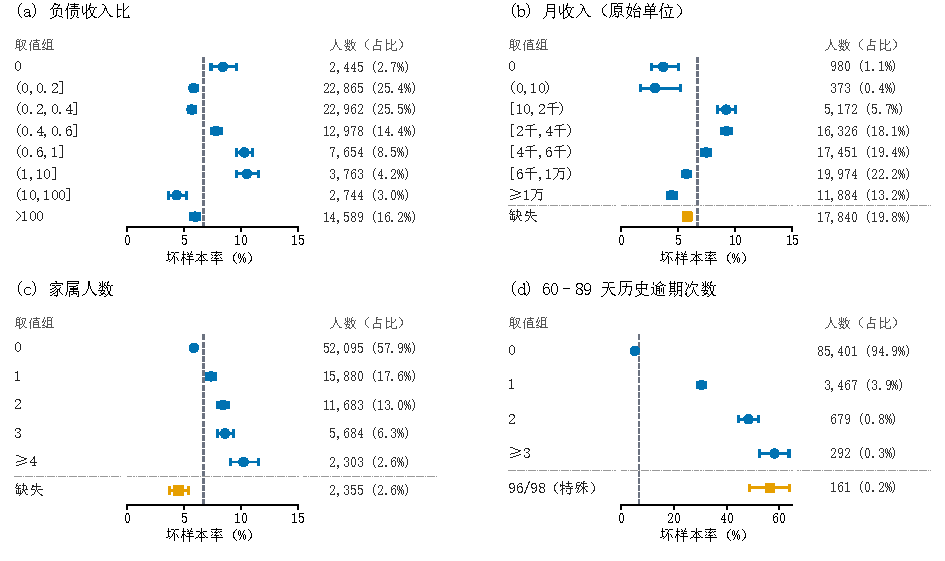
\includegraphics{figures/feature_risk.pdf}
  \small
  \caption{四变量的训练集分布与边际风险}
  \label{fig:training-feature-risk}
  \begin{minipage}{\linewidth}
    \footnotesize
    注：点为坏样本率，横线为记录层面的 Wilson 95\% 二项比例区间，
    右列为人数及占全部训练样本的比例。虚线为训练集总体坏样本率，
    方块标记缺失或 96/98 特殊组；各面板横轴范围不同。
  \end{minipage}
\end{figure}

\subsection{异常值和缺失值处理}
\label{sec:preprocessing}
% !TeX root = ../main.tex
\newcommand{\PreprocessAgeMedian}{52}
\newcommand{\PreprocessAgeChanged}{1}
\newcommand{\PreprocessTrainN}{90,000}
\newcommand{\PreprocessValidationN}{30,000}
\newcommand{\PreprocessTestN}{30,000}


按家属人数、逾期编码、收入状态依次处理，标记允许重叠，规则见表~\ref{tab:cleaning-rules}。
相较于无标记的直接填补，保留指示或独立状态可避免混同图~\ref{fig:training-feature-risk} 中风险不同的人群；
本节选定数据准备方案，预测性能仍由后续验证比较。

\begin{table}[!htbp]
  \centering
  \caption{缺失与特殊值的冻结处理规则}
  \label{tab:cleaning-rules}
  \footnotesize
  \setlength{\tabcolsep}{3pt}
  \renewcommand{\arraystretch}{1.04}
  \begin{tabular}{p{2.0cm}p{13.1cm}}
    \toprule
    对象 & 处理及迁移规则 \\
    \midrule
    家属人数 & 原缺失先标记为 1 再补 0，原生零值标记为 0，保留两类差异。 \\
    三类逾期 & 保留原值，逐列标记 96/98 并合为该变量的特殊档；共同标记仅追踪任一列命中，避免重复计人数。 \\
    月收入 & 保留原值；缺失、$[0,10)$、$[10,+\infty)$ 分别为 \texttt{MISSING}、\texttt{LOW}、\texttt{REGULAR}。
    前两者路由特殊档，10 归普通档，原 NA 由缺失状态映射。 \\
    年龄 & 缺失或不大于 0 时补训练集有效年龄中位数 \PreprocessAgeMedian{} 岁并标记。
    本次改动 \PreprocessAgeChanged{} 条；训练中恒定的异常标记仅供审计，不估计系数。 \\
    比例与长尾 & DebtRatio 在各收入状态下保留；比例大于 1、高收入及其他合法长尾均不截尾或删行，普通分箱和 WOE 留待模块三学习。 \\
    \bottomrule
  \end{tabular}
\end{table}

\begin{samepage}
\paragraph{家属人数缺失的处理依据}
在完整训练集中，家属人数缺失组的坏样本率为 \DependentsMissingRisk，原生零值组为
\DependentsZeroRisk，均低于家属人数为正组的 8.08\%，呈现相对较低的边际风险。
因此，选择 0 作为缺失记录的数值占位，同时保留原缺失指示，使其在数值表示上与零值组衔接，
并允许后续模型识别缺失状态的附加信息。这一处理不将两组风险视为相同，
也不认定缺失客户的真实家属人数为 0；相较于直接补 0，缺失标记保留了两类记录的区别。\par
\end{samepage}

\paragraph{逾期特殊编码的保留依据}
三类逾期字段的 96/98 在训练集中命中同一批 \LateSpecialN{} 条记录，其中 91 条为坏样本，
坏样本率达 \LateSpecialRisk，明显高于训练集总体的 6.68\%。
该编码状态具有较强的样本风险区分信息，直接删除会丢失目标事件高度集中的记录。
鉴于公开字典未明确其业务含义，本研究保留原始记录，将 96/98 合并为特殊档，
既保留其风险信息，也避免将未知编码当作正常逾期次数排序。
其中 96 仅有 2 条训练记录，与 98 合并可避免对极稀疏子组单独估计风险；
三列共享的特殊状态在联合建模时仍需检查重复信息。
\paragraph{收入三种状态的划分依据}
为考察非逾期特殊编码人群中的收入关系，在不含 96/98 的 89,839 条训练记录中比较：
收入缺失、$[0,10)$ 及 $[10,+\infty)$ 三组分别有 17,768、1,347、70,724 条，
坏样本率分别为 5.57\%、3.34\%、6.91\%。
缺失与极低收入组不仅区别于普通收入组，彼此也呈现不同的边际风险，
因此分别设置 \texttt{MISSING} 和 \texttt{LOW} 状态，避免预先合并，
普通收入组再于后续学习常规分箱。这是基于记录状态与风险分布的编码选择，
并不意味着收入越低越安全。上述条件样本仅用于解释收入分层，实际转换仍覆盖所有记录，
包括命中 96/98 的客户，收入状态与逾期标记可以重叠。

数据处理后，三个子集的样本个数不变。
参数只从训练特征估计，冻结后统一用于验证、测试及新客户；交叉验证在折内重估。
合法超训练范围值保留，由后续开口箱覆盖；缺字段、非法格式、无穷值、负收入或比例、
负或非整数计数及未约定缺失均报字段级错误，不静默删行。
新客户无需标签；完整规则清单、变动人数和标记重叠记录随代码保存。


\section{分箱、WOE 与 IV}
\subsection{分箱方案}
\label{sec:binning}
% !TeX root = ../main.tex

在第~\ref{sec:preprocessing}~节处理结果上，结合变量定义、训练集分布与已观察的风险关系，
确定表~\ref{tab:initial-binning} 的初始分箱方案。连续变量采用便于解释的业务边界，
离散计数保留低次数差异并合并稀疏尾部；缺失及未知特殊编码优先按既定规则路由。
各变量独立分箱，同一客户可以同时属于收入特殊档和某逾期字段的特殊档，保留全部记录。

\begin{table}[!htbp]
  \centering
  \caption{十个原始特征的初始分箱方案}
  \label{tab:initial-binning}
  \footnotesize
  \setlength{\tabcolsep}{3pt}
  \renewcommand{\arraystretch}{1.12}
  \begin{tabular}{>{\raggedright\arraybackslash}p{2.2cm}>{\raggedright\arraybackslash}p{8.0cm}>{\raggedright\arraybackslash}p{4.3cm}}
    \toprule
    特征 & 候选分箱 & 主要考虑 \\
    \midrule
    循环额度使用率 & $0$；$(0,0.1]$；$(0.1,0.3]$；$(0.3,0.6]$；$(0.6,1]$；$(1,+\infty)$ & 零使用率单列；保留超额度状态。 \\
    年龄 & $(0,30)$；$[30,40)$；$[40,50)$；$[50,60)$；$[60,70)$；$[70,+\infty)$ & 按年龄段划分，考察风险随年龄的变化。 \\
    30--59 天逾期次数 & $0$；$1$；$2$；$3$；普通值 $\geq4$；96/98 特殊档 & 区分首次与重复逾期，合并普通高次数尾部。 \\
    负债收入比 & $0$；$(0,0.4]$；$(0.4,0.6]$；$(0.6,1]$；$(1,10]$；$(10,100]$；$(100,+\infty)$ & 保留 1 的业务边界及非单调尾部。 \\
    月收入 & 缺失；$[0,10)$；$[10,4{,}000)$；$[4{,}000,6{,}000)$；$[6{,}000,10{,}000)$；$[10{,}000,+\infty)$ & 前两档为既定特殊状态，普通收入再分层。 \\
    开放信贷账户数 & $0$；$1$--$2$；$3$--$5$；$6$--$9$；$10$--$14$；$\geq15$ & 兼顾信贷经历不足与账户较多的不同含义。 \\
    90 天及以上逾期次数 & $0$；$1$；$2$；普通值 $\geq3$；96/98 特殊档 & 保留严重逾期次数的风险梯度。 \\
    房地产贷款或额度数 & $0$；$1$--$2$；$3$；$\geq4$ & 区分无此类贷款、少量持有及较多持有。 \\
    60--89 天逾期次数 & $0$；$1$；普通值 $\geq2$；96/98 特殊档 & 普通 $\geq3$ 次仅 292 人，先与 2 次合并。 \\
    家属人数 & $0$；$1$；$2$；$3$；$\geq4$ & 基于填补后数值分箱，另保留原缺失指示。 \\
    \bottomrule
  \end{tabular}
\end{table}

\paragraph{分箱约束与标记用途}
普通箱以训练样本数不少于 450（训练集的 0.5\%）、好坏样本各不少于 30 作为初步检查标准，
结合相邻风险差异与业务含义决定是否合并。
具有明确识别规则的特殊档（例如借款人的三类逾期 96/98 编码）可保留较小样本规模。
家属人数的零值箱包含原生零值及缺失后补零的记录，
同时将 \texttt{NumberOfDependents\_missing} 的 0/1 两档作为候选输入，保留缺失信息。

\paragraph{DebtRatio 尾部分档的依据}
字典将 DebtRatio 定义为每月债务偿付、赡养费和生活费用与月总收入之比。
因此，大于 1 表示这些支出超过当月收入，提示负担较重、需要进一步核查，不能仅据此判为错误。
表~\ref{tab:initial-binning} 中大于 1 的各档仍为普通数值档，与未知编码的特殊档含义不同。
图~\ref{fig:training-feature-risk} 显示，坏样本率由 $(0.2,0.4]$ 档的 5.65\%
上升至 $(0.4,0.6]$、$(0.6,1]$ 和 $(1,10]$ 档的 7.81\%、10.28\% 和 10.50\%，
随后在 $(10,100]$ 和大于 100 档降至 4.34\% 和 5.97\%。
两个尾部档分别有 2,744 和 14,589 人，不能将其下降简单归为极少数记录造成的波动。

交叉统计进一步发现，大于 100 的 14,589 人中，收入缺失、为零和大于零但低于 10 的人数
分别为 13,586、724 和 276，三组合计 14,586 人，占 99.98\%；
相应坏样本率分别为 6.14\%、4.01\% 和 2.90\%。
DebtRatio 大于 1 后，各区间的坏样本率差异明显，且未呈现单调变化；极高值又集中于收入缺失或极低的样本，
不能简单理解为比率越大、风险越高。因此，保留这些区间分别分箱，避免强行合并掩盖风险差异，
后续再结合收入状态和验证集表现决定是否调整。


\subsection{WOE 与 IV 编码}
\label{sec:woe}
% !TeX root = ../main.tex

以固定训练集的 $N_0=83{,}984$ 个好样本和 $N_1=6{,}016$ 个坏样本计算编码。
对某变量的第 $k$ 档，记好、坏样本数为 $n_{0k}$、$n_{1k}$，总档数为 $K$，
其中缺失、低收入及 96/98 等已定义的特殊档均计入 $K$。
两类样本在各档的平滑分布为：
\begin{equation}
  g_k=\frac{n_{0k}+\alpha}{N_0+\alpha K},\qquad
  b_k=\frac{n_{1k}+\alpha}{N_1+\alpha K},\qquad \alpha=0.5.
  \label{eq:smoothed-distributions}
\end{equation}

WOE 统一采用好样本分布除以坏样本分布：

\begin{equation}
  \mathrm{WOE}_k=\ln\frac{g_k}{b_k}.
  \label{eq:woe}
\end{equation}

因此，正 WOE 表示该档相对更多地聚集好样本，负 WOE 表示相对更多地聚集坏样本。
逐档 IV 贡献及变量总 IV 定义为
\begin{equation}
  \mathrm{IV}_k=(g_k-b_k)\ln\frac{g_k}{b_k},\qquad
  \mathrm{IV}=\sum_{k=1}^{K}\mathrm{IV}_k.
  \label{eq:iv}
\end{equation}

本报告选择列出\texttt{DebtRatio}和\texttt{NumberOfTimes90DaysLate}的分箱结果,
详见表~\ref{tab:debt-woe}、表~\ref{tab:late90-woe}
；其余变量的全表保存在配套 CSV 中。
第~\ref{sec:binning}~节方案执行后，各变量档数与该节初始设计一致，本轮未再次合并。
全部普通档人数至少为 779，好、坏样本数分别至少为 287、106，均通过预定要求。
96/98 档共 161 人，作为未知编码的特殊状态独立保留。

\begin{table}[!htbp]
  \centering
  \caption{DebtRatio 的完整训练分箱表}
  \label{tab:debt-woe}
  \footnotesize
  \setlength{\tabcolsep}{2.2pt}
  \renewcommand{\arraystretch}{1.05}
  \begin{tabular}{lrrrrrrrr}
\toprule
档位 & 人数 & 好 & 坏 & 坏率 & $g_k$ & $b_k$ & WOE & IV 贡献 \\
\midrule
$0$ & 2,445 & 2,240 & 205 & 8.38\% & 0.02668 & 0.03414 & -0.2467 & 0.00184 \\
$(0,0.4]$ & 45,827 & 43,201 & 2,626 & 5.73\% & 0.51438 & 0.43633 & 0.1646 & 0.01284 \\
$(0.4,0.6]$ & 12,978 & 11,965 & 1,013 & 7.81\% & 0.14247 & 0.16837 & -0.1670 & 0.00433 \\
$(0.6,1]$ & 7,654 & 6,867 & 787 & 10.28\% & 0.08177 & 0.13082 & -0.4700 & 0.02306 \\
$(1,10]$ & 3,763 & 3,368 & 395 & 10.50\% & 0.04011 & 0.06570 & -0.4936 & 0.01263 \\
$(10,100]$ & 2,744 & 2,625 & 119 & 4.34\% & 0.03126 & 0.01985 & 0.4540 & 0.00518 \\
$(100,+\infty)$ & 14,589 & 13,718 & 871 & 5.97\% & 0.16334 & 0.14478 & 0.1206 & 0.00224 \\
\midrule
合计 & 90,000 & 83,984 & 6,016 & 6.68\% & 1 & 1 & --- & 0.06212 \\
\bottomrule
\end{tabular}

\end{table}

\begin{table}[!htbp]
  \centering
  \caption{NumberOfTimes90DaysLate 的完整训练分箱表}
  \label{tab:late90-woe}
  \footnotesize
  \setlength{\tabcolsep}{2.2pt}
  \renewcommand{\arraystretch}{1.05}
  \begin{tabular}{lrrrrrrrr}
\toprule
档位 & 人数 & 好 & 坏 & 坏率 & $g_k$ & $b_k$ & WOE & IV 贡献 \\
\midrule
$0$ & 84,989 & 81,057 & 3,932 & 4.63\% & 0.96513 & 0.65340 & 0.3901 & 0.12159 \\
$1$ & 3,159 & 2,094 & 1,065 & 33.71\% & 0.02494 & 0.17704 & -1.9599 & 0.29811 \\
$2$ & 912 & 476 & 436 & 47.81\% & 0.00567 & 0.07253 & -2.5481 & 0.17035 \\
$\geq 3$ & 779 & 287 & 492 & 63.16\% & 0.00342 & 0.08183 & -3.1741 & 0.24887 \\
96/98（特殊） & 161 & 70 & 91 & 56.52\% & 0.00084 & 0.01520 & -2.8965 & 0.04161 \\
\midrule
合计 & 90,000 & 83,984 & 6,016 & 6.68\% & 1 & 1 & --- & 0.88053 \\
\bottomrule
\end{tabular}

\end{table}

\paragraph{一档独立核算}
DebtRatio 的 $(1,10]$ 档有 3,368 个好样本、395 个坏样本，变量共 $K=7$ 档。
将人数直接代入式~\eqref{eq:smoothed-distributions}--\eqref{eq:iv}：
\begin{equation}
  \begin{aligned}
    g_k&=\frac{3{,}368+0.5}{83{,}984+0.5\times7}=0.0401072,\qquad
    b_k=\frac{395+0.5}{6{,}016+0.5\times7}=0.0657031,\\
    \mathrm{WOE}_k&=\ln\!\left(\frac{0.0401072}{0.0657031}\right)\approx-0.4936,\qquad
    \mathrm{IV}_k\approx0.01263.
  \end{aligned}
  \label{eq:woe-hand-check}
\end{equation}

该档占全部坏样本的比例高于其占全部好样本的比例，因而 WOE 为负；
其档内坏样本率 10.50\% 也高于训练集总体的 6.68\%。
图~\ref{fig:woe-debt-late90} 展示各档编码：严重逾期的普通档随次数增加而 WOE 下降，
DebtRatio 则保留前文解释的非单调关系，96/98 不参与普通次数的排序。

\begin{figure}[!htbp]
  \centering
  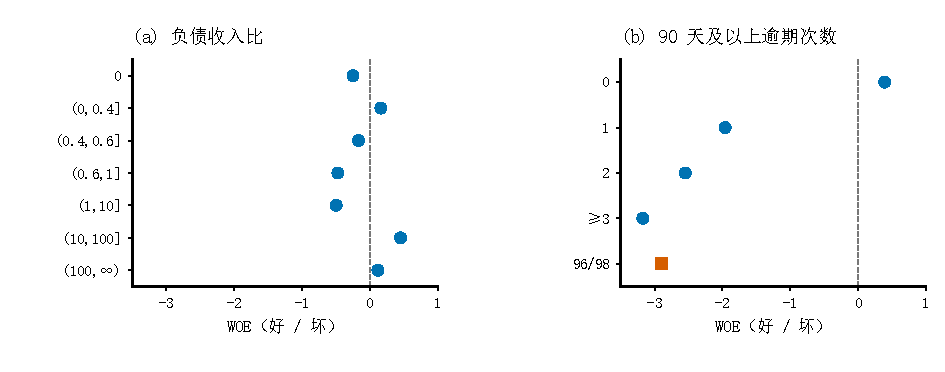
\includegraphics{figures/woe_debt_late90.pdf}
  \small
  \caption{DebtRatio 与历史严重逾期的 WOE 分布}
  \label{fig:woe-debt-late90}
  \begin{minipage}{\linewidth}
    \footnotesize
    注：点为训练集平滑 WOE，圆点为普通档，方块为 96/98 特殊档，虚线表示 WOE 为 0。
  \end{minipage}
\end{figure}

\paragraph{编码冻结与迁移}
保存切点、开闭端点、特殊路由和训练 WOE，验证客户按同一规则查表，
后续测试及新客户也使用该映射，不根据其标签重新计算编码。
若在训练集内部进行交叉验证，数据驱动的切点设计、预处理、WOE 和变量选择均须在各训练折内重做。

\subsection{候选变量的选择}
\label{sec:feature-selection}
% !TeX root = ../main.tex

候选输入包括十个原始变量和家属人数原缺失指示，共 11 项。
表~\ref{tab:iv-candidates} 按训练 IV 排序。
IV 衡量单个变量在当前分箱下的边际区分能力，不代表进入联合模型后的独立贡献，
也不要求风险关系单调。故以 IV 确定检查优先级，再结合字段时点、档量、冗余与验证表现作取舍。

\begin{table}[!htbp]
  \centering
  \caption{候选变量的训练集 IV 与初选结果}
  \label{tab:iv-candidates}
  \footnotesize
  \setlength{\tabcolsep}{3.5pt}
  \renewcommand{\arraystretch}{1.05}
  \begin{tabular}{lrrrrl}
\toprule
候选变量 & 档数 & 最小档人数 & IV & 特殊档 IV 占比 & 初选 \\
\midrule
额度使用率 & 6 & 1,973 & 1.1293 & --- & 保留 \\
90 天及以上逾期次数 & 5 & 161 & 0.8805 & 4.7\% & 保留 \\
30–59 天逾期次数 & 6 & 161 & 0.7805 & 5.3\% & 保留 \\
60–89 天逾期次数 & 4 & 161 & 0.5832 & 7.1\% & 保留 \\
年龄 & 6 & 5,248 & 0.2513 & --- & 保留 \\
在用信贷账户数 & 6 & 1,119 & 0.1016 & --- & 暂不纳入 \\
月收入 & 6 & 1,353 & 0.0730 & 13.5\% & 暂不纳入 \\
负债收入比 & 7 & 2,445 & 0.0621 & --- & 保留 \\
房地产贷款数 & 4 & 2,179 & 0.0589 & --- & 保留 \\
家属人数 & 5 & 2,303 & 0.0364 & --- & 保留 \\
家属人数原缺失指示 & 2 & 2,355 & 0.0038 & --- & 暂不纳入 \\
\bottomrule
\end{tabular}

  \begin{minipage}{\linewidth}
    \footnotesize
    注：最小档人数包含特殊档；特殊档 IV 占比为其贡献之和除以变量总 IV。
    三类逾期的特殊档均为 96/98，月收入的特殊档为缺失及 $[0,10)$。
    初选结果同时使用表~\ref{tab:candidate-validation} 的联合诊断，不按 IV 阈值直接删除。
  \end{minipage}
\end{table}

\paragraph{高 IV 的来源与字段时点}
对于额度使用率和三类逾期的 IV 均超过 0.5的候选变量，需要核查其区分信息是否依赖稀疏档或未来信息。
额度使用率的最小档有 1,973 人；三类逾期普通档最少分别有 805、971、779 人
（依次为 30--59、60--89、90 天及以上），并无零好样本或零坏样本档。
96/98 对三类逾期总 IV 的贡献占比分别仅为 5.3\%、7.1\%、4.7\%，
说明高 IV 主要来自普通逾期记录的分布差异，不能归因于这 161 人的特殊编码。
因此，额度使用率和三类历史逾期变量均保留为候选变量。

\paragraph{候选变量方案确定}
为判断候选变量在联合模型中是否仍提供额外信息，使用相同设置的 Logistic 模型比较不同变量组合，
结果见表~\ref{tab:candidate-validation}。完整 11 项方案作为参照，比较按 IV 阈值筛选
及综合筛选后的验证表现。

\begin{table}[!htbp]
  \centering
  \caption{候选变量方案的验证集诊断表现}
  \label{tab:candidate-validation}
  \footnotesize
  \setlength{\tabcolsep}{5pt}
  \renewcommand{\arraystretch}{1.05}
  \begin{tabular}{lrrrrr}
\toprule
诊断方案 & 变量数 & AUC & KS & 对数损失 & Brier \\
\midrule
全部 11 项 & 11 & 0.8639 & 0.5692 & 0.18130 & 0.04997 \\
仅 IV $\geq0.02$ & 10 & 0.8639 & 0.5690 & 0.18129 & 0.04996 \\
仅 IV $\geq0.10$ & 6 & 0.8598 & 0.5666 & 0.18245 & 0.05012 \\
综合初选方案 & 8 & 0.8636 & 0.5678 & 0.18138 & 0.04997 \\
\bottomrule
\end{tabular}

\end{table}

\paragraph{8 项初选方案的形成过程}
完整模型先纳入全部 11 项，然后依训练 IV 由小到大逐项试删，每次删除后重新拟合模型并计算验证指标。
候选变量简化统一基准：AUC 最多减少 0.001，
对数损失和 Brier 最多各增加 0.0001，三项同时满足才简化；KS 用作辅助观察。
这些差异界限是本研究预设的简化标准，不是统计显著性检验。
实际通过检查的三次删除见表~\ref{tab:accepted-removals}，其间其他变量的试删未通过，故继续保留。

\begin{table}[!htbp]
  \centering
  \caption{从 11 项到 8 项的已接受删选步骤}
  \label{tab:accepted-removals}
  \footnotesize
  \setlength{\tabcolsep}{4pt}
  \renewcommand{\arraystretch}{1.05}
  \begin{tabular}{lrrrrr}
    \toprule
    当前组合 & 项数 & AUC & KS & 对数损失 & Brier \\
    \midrule
    完整方案 & 11 & 0.863872 & 0.569176 & 0.181303 & 0.049968 \\
    去掉家属人数缺失指示 & 10 & 0.863898 & 0.568997 & 0.181289 & 0.049961 \\
    再去掉月收入 & 9 & 0.863562 & 0.567191 & 0.181372 & 0.049967 \\
    再去掉在用信贷账户数 & 8 & 0.863584 & 0.567834 & 0.181375 & 0.049965 \\
    \bottomrule
  \end{tabular}
  \begin{minipage}{\linewidth}
    \footnotesize
  \end{minipage}
\end{table}

家属人数原缺失指示的 IV 为 0.0038，单独区分能力较弱；
从完整模型中去掉它后，符合上文提到的简化条件。

月收入的 IV 为 0.0730，尽管其具有一定的单变量信息，但数据发现，
在去掉家属人数缺失指示的基础上，再去掉月收入，AUC 从 0.863898 降至 0.863562，
对数损失从 0.181289 升至 0.181372，但相对完整方案的差异仍在上述界限内。
另一方面，本数据中该字段的信息完整性有限：训练集约 19.82\%的收入缺失，
另有约 1.50\%的收入低于 10，两类合计约占 21.33\%。
这些记录虽已通过特殊分箱保留状态信息，却难以直接解释为客户的正常收入水平。

在用信贷账户数的 IV 为 0.1016，但在上述 9 项组合中去掉它，
符合上文提到的简化条件，当前联合预测中仍可省略。
三个变量的取舍均依据实际试删结果，而非达到或未达到某个 IV 阈值。

由此，进入模块四的 8 项候选为额度使用率、年龄、三类历史逾期次数、
DebtRatio、房地产贷款数和家属人数。该组合以较少输入取得接近完整方案的验证表现，
是本次顺序筛选的初选结果；最终效果仍在模型冻结后通过测试集评价。


\section{Logistic 建模与比较基准}
\label{sec:logistic}
% !TeX root = ../main.tex
\newcommand{\LogitWoeIterations}{30}
\newcommand{\LogitRawIterations}{17}
\newcommand{\LogitMaxVIF}{1.25}
\newcommand{\LogitCondition}{1.83}
\newcommand{\LogitTrainingRate}{6.6844\%}

\begingroup
\setlength{\intextsep}{7pt}
\setlength{\textfloatsep}{10pt}

\subsection{模型估计与诊断}
将第~\ref{sec:feature-selection}~节的 8 项冻结 WOE 输入模型，以坏样本为正类：
\begin{equation}
  Y_i\mid\boldsymbol{x}_i\sim\mathrm{Bernoulli}(p_i),\qquad
  \eta_i=\log\frac{p_i}{1-p_i}=\beta_0+\sum_{j=1}^{8}\beta_jw_j(x_{ij}).
  \label{eq:woe-logistic}
\end{equation}
概率为 $p_i=(1+e^{-\eta_i})^{-1}$。按记录采用条件独立的工作假设，重复与同源限制沿用第~\ref{sec:sample-split}~节；
条件对数几率对 WOE 加性，无需八个特征相互独立。固定 $C=1$，以无类别权重的 L2 惩罚估计
\begin{equation}
  \widehat{\boldsymbol\beta}
  =\arg\min_{\boldsymbol\beta}\left\{
    \sum_{i\in\mathcal T}\bigl[\log(1+e^{\eta_i})-Y_i\eta_i\bigr]
    +\frac{1}{2C}\sum_{j=1}^{8}\beta_j^2\right\},
  \label{eq:penalized-logistic}
\end{equation}
其中 $\mathcal T$ 为训练集，截距不惩罚。采用 \texttt{lbfgs}数值优化算法、容差 $10^{-8}$、最多 2,000 次迭代，
在 \LogitWoeIterations{} 次后收敛。含截距的标准化诊断矩阵秩为 9、条件数为 \LogitCondition，最大 VIF 为 \LogitMaxVIF。
后可根据此惩罚估计得到八个候选变量的WOE Logistic的估计系数。

\begin{table}[!htbp]
  \centering
  \caption{八变量 WOE Logistic 的估计系数}
  \label{tab:logistic-coefficients}
  \footnotesize
  \setlength{\tabcolsep}{8pt}
  \renewcommand{\arraystretch}{1.02}
  \begin{tabular}{lrr}
\toprule
项 & 系数 $\widehat\beta$ & $\exp(\widehat\beta)$ \\
\midrule
截距 & -2.60255 & 0.0741 \\
额度使用率 & -0.61583 & 0.5402 \\
年龄 & -0.40832 & 0.6648 \\
30–59 天逾期次数 & -0.51178 & 0.5994 \\
负债收入比 & -0.76611 & 0.4648 \\
90 天及以上逾期次数 & -0.53753 & 0.5842 \\
房地产贷款数 & -0.67415 & 0.5096 \\
60–89 天逾期次数 & -0.35875 & 0.6986 \\
家属人数 & -0.28302 & 0.7535 \\
\bottomrule
\end{tabular}

  \begin{minipage}{\linewidth}
    \footnotesize
    注：非截距行的指数表示其他 WOE 固定时，该变量增加 1 个 WOE 单位的坏样本几率比；
    截距项的指数表示所有 WOE 为 0 时的坏/好几率。
  \end{minipage}
\end{table}

表~\ref{tab:logistic-coefficients} 八项系数均为负：WOE 增大时条件坏样本几率下降。
以负债收入比为例，当其他七项 WOE 不变时，负债收入比的 WOE 增加 1 个单位，
坏样本几率变为原来的 0.5402 倍，即降低约 45.98\%。
年龄系数的单位也是 WOE，并非每增加一岁的效应，截距不代表平均客户风险。

\subsection{具体档位的条件几率比}
同一变量由档位 $a$ 变为 $b$，其余七项输入固定时，
\begin{equation}
  \mathrm{OR}_{b:a}
  =\frac{p_b/(1-p_b)}{p_a/(1-p_a)}
  =\exp\!\left\{\widehat\beta_j\bigl(w_{j,b}-w_{j,a}\bigr)\right\}.
  \label{eq:conditional-bin-odds-ratio}
\end{equation}

以第~\ref{sec:scorecard}~节的低风险人工输入为参照。负债收入比分别设为 0.25 与 2，严重逾期次数分别设为 0 与 1。
分别只改设负债比或严重逾期档位，结果见表~\ref{tab:logistic-odds-examples}。
DebtRatio 的 WOE 差为 $-0.65815$，与系数 $-0.76611$ 结合得到 $\mathrm{OR}\approx1.656$；
严重逾期的 WOE 差为 $-2.35001$，与系数 $-0.53753$ 结合得到 $\mathrm{OR}\approx3.537$。
几率倍数不等于概率倍数；概率变化依赖参照特征，表示模型情景比较，不解释为因果效应。

\begin{table}[!htbp]
  \centering
  \caption{固定其余特征后的档位比较}
  \label{tab:logistic-odds-examples}
  \footnotesize
  \setlength{\tabcolsep}{6pt}
  \begin{tabular}{llrrr}
\toprule
变量 & 档位变化 $a\to b$ & 条件几率比 & $p_a$ & $p_b$ \\
\midrule
负债收入比 & $(0,0.4]\to(1,10]$ & 1.656 & 1.13\% & 1.85\% \\
90 天及以上逾期次数 & $0\to1$ & 3.537 & 1.13\% & 3.88\% \\
\bottomrule
\end{tabular}

\end{table}

\subsection{两个基准与同样本比较}
\paragraph{常数概率基准}
对所有客户预测训练集坏样本率 $\widehat p_0=6{,}016/90{,}000=\LogitTrainingRate$，
不从测试标签重估先验。
\paragraph{原始字段 Logistic 基准}
同样八个字段中，年龄保留原值，其余取 $\log(1+x)$。
96/98 对应普通计数置 0，以单个“任一逾期特殊”指示保留状态，共 9 个设计量，避免三个相同标记重复输入。
按训练均值和总体标准差缩放后冻结，使用同一 $C$、求解器及无权重设置，
17 次后收敛，矩阵满列秩且未检出分离。

两模型参数和规则先冻结，随后才打开同一批 30,000 条测试记录（坏样本 2,005 条），结果见表~\ref{tab:logistic-comparison}。
两个 Logistic 模型采用相同的八个原始字段，分别使用数值变换后的原值表示和分箱后的 WOE 表示。
测试结果显示，WOE 流程的 AUC 提高约 0.0235，KS 和 AP 同时提高，
对数损失与 Brier 分别降低约 4.53\%和 2.91\%，
表明该流程在本次实验中改善了风险排序与整体概率预测质量。
这与分箱能够表达不同取值区间的风险差异相一致，例如 DebtRatio 的非单调关系难以通过单一对数变换充分表达。

\paragraph{不平衡与准确率}
训练沿用约 $13.96:1$ 的好坏比，各记录等权。给定模型预测的坏样本概率 $\widehat p_i$，
记分类阈值为 $t$，由此定义预测标签
\[
  \widehat Y_i(t)=
  \begin{cases}
    1,\ \text{标记为高风险客户}, & \widehat p_i\geq t,\\
    0,\ \text{不标记为高风险客户}, & \widehat p_i<t.
  \end{cases}
\]

若误报与漏报代价相同且预测概率可信，标记和不标记的期望成本分别与
$1-\widehat p_i$ 和 $\widehat p_i$ 成正比。当 $1-\widehat p_i\leq\widehat p_i$ 时选择标记，
得到等代价对照阈值 $t_0=0.5$。（即此时考虑误报好客户成本与漏报坏客户成本相同）

以坏样本为正类，将 WOE 模型的 $\widehat Y_i(t_0)$ 与测试集实际标签逐一比较，
得到正确检出 $TP=364$、漏报 $FN=1{,}641$、误报 $FP=244$、正确识别好客户 $TN=27{,}751$。
准确率与坏样本召回率的定义及代入结果分别为
\[
  \begin{gathered}
    \mathrm{Accuracy}(t)=\frac{TP(t)+TN(t)}{N},\qquad
    \mathrm{Recall}_{\mathrm{bad}}(t)=\frac{TP(t)}{TP(t)+FN(t)},\\[0.3ex]
    \mathrm{Accuracy}(t_0)=\frac{364+27{,}751}{30{,}000}=93.72\%,\qquad
    \mathrm{Recall}_{\mathrm{bad}}(t_0)=\frac{364}{2{,}005}=18.15\%.
  \end{gathered}
\]

在该阈值下，好样本识别率为 99.13\%。常数基准的预测概率低于 $t_0$，因而将所有人判为好样本，
准确率等于好样本占比 93.32\%，坏样本召回率为 0。好样本数量占优，使总体准确率主要反映多数类的识别表现。

\endgroup


\section{评分刻度与标准评分卡}
\label{sec:scorecard}
% !TeX root = ../main.tex
\newcommand{\ScoreA}{515.041450}
\newcommand{\ScoreB}{28.853901}
\newcommand{\ScoreIntercept}{590.135076}
\newcommand{\ScoreMaxRoundError}{2.123}
\newcommand{\ScoreMaxProbabilityError}{6.11e-16}
\newcommand{\ScoreCardBins}{43}

\begingroup
\setlength{\intextsep}{6pt}
\setlength{\textfloatsep}{9pt}
\setlength{\abovedisplayskip}{6pt}
\setlength{\belowdisplayskip}{6pt}
\setlength{\abovedisplayshortskip}{3pt}
\setlength{\belowdisplayshortskip}{5pt}

\subsection{刻度推导与分数分解}
设坏样本概率为 $p\in(0,1)$，好坏几率为 $O=\frac{1-p}{p}$，评分函数为 $S=A+B\ln O$。
几率翻倍时分差为 $B[\ln(2O)-\ln O]=20$，且 $A+B\ln 19=600$，得到
\begin{equation}
  B\ln 2=20,\qquad B=\frac{20}{\ln 2}\approx\ScoreB,\qquad
  A=600-B\ln 19\approx\ScoreA.
  \label{eq:score-scaling}
\end{equation}
概率与分数之间的转换为
\begin{equation}
  S(p)=A+B\ln\frac{1-p}{p},\qquad
  p(S)=\frac{1}{1+\exp\!\left(\frac{S-A}{B}\right)}.
  \label{eq:score-probability}
\end{equation}
令 $\widehat\eta_i$ 为式~\eqref{eq:woe-logistic} 的拟合对数几率。代入后可分解客户 $i$ 的总分
\begin{equation}
  S_i=A-B\widehat\eta_i=S_0+\sum_{j=1}^{8}s_j(x_{ij}),\qquad
  S_0=A-B\widehat\beta_0,\qquad s_j(x_{ij})=-B\widehat\beta_j w_j(x_{ij}).
  \label{eq:score-decomposition}
\end{equation}
评分锚点由 $O=19$ 给定，即 $p=\tfrac{1}{20}=5\%$ 时 $S=600$。令八项 WOE 均为零，
则截距取值 $b$ 对应基准概率 $p_0(b)=(1+\exp(-b))^{-1}$ 和基准分 $S_0(b)=A-Bb$，因此
\[
  \begin{aligned}
    b=0 &\quad\Longrightarrow\quad p_0(0)=50\%,\qquad S_0(0)=A\approx\ScoreA,\\
    \widehat\beta_0\approx-2.602547 &\quad\Longrightarrow\quad
    p_0(\widehat\beta_0)\approx6.8975\%,\qquad S_0(\widehat\beta_0)\approx\ScoreIntercept.
  \end{aligned}
\]
由于 $\widehat\eta_i$ 随坏样本概率严格递增，$B>0$ 时坏样本概率越高，分数越低。
对同一模型采用新刻度 $S_i'=A'-B'\widehat\eta_i$（$B'>0$），任意两位客户 $i,k$ 满足
\[
  S_i'-S_k'=-B'(\widehat\eta_i-\widehat\eta_k)=\frac{B'}{B}(S_i-S_k).
\]
截距 $A'$ 在分差中抵消，$B'/B$ 为正，分差的正、负和零均保持，因此未取整分数的先后与并列关系均保持。

\subsection{完整评分卡}
表~\ref{tab:complete-scorecard} 包含全部 \ScoreCardBins{} 档及独立基准分。
整数展示对基准分和八项档分各取最近整数，恰好半分时远离 0，再相加；
它不一定等于总分最后一次取整。计算及阈值评价均使用未取整分数，不截断分值。
表中分值未取整，仅显示三位小数，完整精度另存 \texttt{scorecard.csv}。

\begin{table}[!htbp]
  \centering
  \caption{完整评分卡}
  \label{tab:complete-scorecard}
  \scriptsize\linespread{1}\selectfont
  \setlength{\tabcolsep}{3pt}
  \renewcommand{\arraystretch}{0.96}
  \begin{minipage}[t]{0.49\linewidth}
\vspace{0pt}
\centering
\begin{tabular}{lrrrr}
\toprule
档位 & WOE & 系数 & 分值 & 整数 \\
\midrule
\multicolumn{5}{l}{\textbf{截距基准分}}\\
基准分 & --- & -2.60255 & 590.135 & 590 \\
\addlinespace[1pt]
\multicolumn{5}{l}{\textbf{额度使用率}}\\
$0$ & 0.73329 & -0.61583 & 13.030 & 13 \\
$(0,0.1]$ & 1.52938 & -0.61583 & 27.176 & 27 \\
$(0.1,0.3]$ & 0.80012 & -0.61583 & 14.217 & 14 \\
$(0.3,0.6]$ & -0.00187 & -0.61583 & -0.033 & 0 \\
$(0.6,1]$ & -1.01802 & -0.61583 & -18.089 & -18 \\
$(1,+\infty)$ & -2.08854 & -0.61583 & -37.112 & -37 \\
\addlinespace[1pt]
\multicolumn{5}{l}{\textbf{年龄}}\\
$(0,30)$ & -0.61527 & -0.40832 & -7.249 & -7 \\
$[30,40)$ & -0.44917 & -0.40832 & -5.292 & -5 \\
$[40,50)$ & -0.25234 & -0.40832 & -2.973 & -3 \\
$[50,60)$ & 0.02838 & -0.40832 & 0.334 & 0 \\
$[60,70)$ & 0.69053 & -0.40832 & 8.136 & 8 \\
$[70,+\infty)$ & 1.09995 & -0.40832 & 12.959 & 13 \\
\addlinespace[1pt]
\multicolumn{5}{l}{\textbf{30–59 天逾期次数}}\\
$0$ & 0.55345 & -0.51178 & 8.173 & 8 \\
$1$ & -0.89868 & -0.51178 & -13.271 & -13 \\
$2$ & -1.62457 & -0.51178 & -23.990 & -24 \\
$3$ & -2.04305 & -0.51178 & -30.170 & -30 \\
$\geq 4$ & -2.42905 & -0.51178 & -35.870 & -36 \\
96/98（特殊） & -2.89647 & -0.51178 & -42.772 & -43 \\
\addlinespace[1pt]
\multicolumn{5}{l}{\textbf{房地产贷款数}}\\
$0$ & -0.22430 & -0.67415 & -4.363 & -4 \\
$1$--$2$ & 0.22561 & -0.67415 & 4.388 & 4 \\
$3$ & -0.04521 & -0.67415 & -0.879 & -1 \\
$\geq 4$ & -0.62112 & -0.67415 & -12.082 & -12 \\
\addlinespace[1pt]
\bottomrule
\end{tabular}
\end{minipage}%
\hfill
\begin{minipage}[t]{0.49\linewidth}
\vspace{0pt}
\centering
\begin{tabular}{lrrrr}
\toprule
档位 & WOE & 系数 & 分值 & 整数 \\
\midrule
\multicolumn{5}{l}{\textbf{负债收入比}}\\
$0$ & -0.24666 & -0.76611 & -5.452 & -5 \\
$(0,0.4]$ & 0.16456 & -0.76611 & 3.638 & 4 \\
$(0.4,0.6]$ & -0.16705 & -0.76611 & -3.693 & -4 \\
$(0.6,1]$ & -0.46997 & -0.76611 & -10.389 & -10 \\
$(1,10]$ & -0.49359 & -0.76611 & -10.911 & -11 \\
$(10,100]$ & 0.45405 & -0.76611 & 10.037 & 10 \\
$(100,+\infty)$ & 0.12062 & -0.76611 & 2.666 & 3 \\
\addlinespace[1pt]
\multicolumn{5}{l}{\textbf{90 天及以上逾期次数}}\\
$0$ & 0.39007 & -0.53753 & 6.050 & 6 \\
$1$ & -1.95995 & -0.53753 & -30.398 & -30 \\
$2$ & -2.54814 & -0.53753 & -39.521 & -40 \\
$\geq 3$ & -3.17409 & -0.53753 & -49.230 & -49 \\
96/98（特殊） & -2.89654 & -0.53753 & -44.925 & -45 \\
\addlinespace[1pt]
\multicolumn{5}{l}{\textbf{60–89 天逾期次数}}\\
$0$ & 0.28407 & -0.35875 & 2.940 & 3 \\
$1$ & -1.81197 & -0.35875 & -18.756 & -19 \\
$\geq 2$ & -2.68735 & -0.35875 & -27.817 & -28 \\
96/98（特殊） & -2.89662 & -0.35875 & -29.984 & -30 \\
\addlinespace[1pt]
\multicolumn{5}{l}{\textbf{家属人数}}\\
$0$ & 0.15601 & -0.28302 & 1.274 & 1 \\
$1$ & -0.10192 & -0.28302 & -0.832 & -1 \\
$2$ & -0.24667 & -0.28302 & -2.014 & -2 \\
$3$ & -0.27142 & -0.28302 & -2.216 & -2 \\
$\geq 4$ & -0.46295 & -0.28302 & -3.781 & -4 \\
\addlinespace[1pt]
\bottomrule
\end{tabular}
\end{minipage}%

\end{table}

\subsection{新客户评分函数与人工案例}
设 $\boldsymbol{x}\in\mathcal X$ 为新客户的十项原始输入。用 $T$ 表示第~\ref{sec:preprocessing}~节的冻结预处理和八项入模变量选取，
令 $\widetilde{x}_j=[T(\boldsymbol{x})]_j$，$w_j(\widetilde{x}_j)$ 为按冻结档位查得的 WOE。
新客户的坏样本概率和未取整总分由下式给出。
\begin{equation}
  \begin{aligned}
    \widehat\eta(\boldsymbol{x})&=\widehat\beta_0+\sum_{j=1}^{8}\widehat\beta_j w_j(\widetilde{x}_j),\\
    \widehat p(\boldsymbol{x})&=\frac{1}{1+\exp[-\widehat\eta(\boldsymbol{x})]},\\
    S(\boldsymbol{x})&=A-B\widehat\eta(\boldsymbol{x})
      =S_0+\sum_{j=1}^{8}\bigl[-B\widehat\beta_j w_j(\widetilde{x}_j)\bigr].
  \end{aligned}
  \label{eq:score-new-customer}
\end{equation}

式中系数、分箱、WOE 和刻度均取已冻结的值。函数 \texttt{score\_customer} 接受包含十项原始字段的字典，
返回 $\widehat p(\boldsymbol{x})$、$S(\boldsymbol{x})$、整数展示分及逐项明细。

构造低、中、高三组人工输入，使用同一冻结评分卡计算。风险标签表示三个案例的相对预测风险。
表~\ref{tab:scorecard-case-detail} 展示八个入模特征的原值、档位、WOE 和档分，
另两项输入与完整计算结果见仓库的 \path{examples/scenarios/}。总分另加基准分 $S_0$。

\begin{table}[H]
  \centering
  \caption{三组人工输入的逐项评分}
  \label{tab:scorecard-case-detail}
  \footnotesize\linespread{1}\selectfont
  \setlength{\tabcolsep}{2pt}
  \renewcommand{\arraystretch}{1.12}
  \newcommand{\casevalue}[2]{\shortstack[r]{$#1$\\[1pt]$#2$}}
  \begin{tabular*}{\linewidth}{@{\extracolsep{\fill}}l*{3}{r>{$}r<{$}>{$}r<{$}}@{}}
    \toprule
    & \multicolumn{3}{c}{低风险}
    & \multicolumn{3}{c}{中风险}
    & \multicolumn{3}{c}{高风险} \\
    \cmidrule(lr){2-4}\cmidrule(lr){5-7}\cmidrule(l){8-10}
    变量 & \shortstack[r]{原值\\档位} & \text{WOE} & \text{档分}
         & \shortstack[r]{原值\\档位} & \text{WOE} & \text{档分}
         & \shortstack[r]{原值\\档位} & \text{WOE} & \text{档分} \\
    \midrule
    额度使用率 & \casevalue{0.08}{(0,0.1]} & 1.52938 & 27.176 & \casevalue{0.35}{(0.3,0.6]} & -0.00187 & -0.033 & \casevalue{0.92}{(0.6,1]} & -1.01802 & -18.089 \\
年龄 & \casevalue{58}{[50,60)} & 0.02838 & 0.334 & \casevalue{35}{[30,40)} & -0.44917 & -5.292 & \casevalue{38}{[30,40)} & -0.44917 & -5.292 \\
30--59 天逾期 & \casevalue{0}{0} & 0.55345 & 8.173 & \casevalue{1}{1} & -0.89868 & -13.271 & \casevalue{2}{2} & -1.62457 & -23.990 \\
负债收入比 & \casevalue{0.25}{(0,0.4]} & 0.16456 & 3.638 & \casevalue{0.3}{(0,0.4]} & 0.16456 & 3.638 & \casevalue{0.57}{(0.4,0.6]} & -0.16705 & -3.693 \\
90 天及以上逾期 & \casevalue{0}{0} & 0.39007 & 6.050 & \casevalue{0}{0} & 0.39007 & 6.050 & \casevalue{2}{2} & -2.54814 & -39.521 \\
房地产贷款数 & \casevalue{1}{1-2} & 0.22561 & 4.388 & \casevalue{1}{1-2} & 0.22561 & 4.388 & \casevalue{0}{0} & -0.22430 & -4.363 \\
60--89 天逾期 & \casevalue{0}{0} & 0.28407 & 2.940 & \casevalue{0}{0} & 0.28407 & 2.940 & \casevalue{1}{1} & -1.81197 & -18.756 \\
家属人数 & \casevalue{0}{0} & 0.15601 & 1.274 & \casevalue{2}{2} & -0.24667 & -2.014 & \casevalue{2}{2} & -0.24667 & -2.014 \\
\bottomrule

  \end{tabular*}
  \par\smallskip
  \parbox{\linewidth}{\scriptsize 原值在上，档位在下。档分显示三位小数，计算使用完整精度。}
\end{table}

\begin{table}[H]
  \centering
  \caption{三组人工输入的总分与概率核验}
  \label{tab:scorecard-case-summary}
  \footnotesize\linespread{1}\selectfont
  \setlength{\tabcolsep}{4pt}
  \renewcommand{\arraystretch}{1.18}
  \begin{tabular*}{\linewidth}{@{\extracolsep{\fill}}l*{6}{>{$}r<{$}}@{}}
    \toprule
    & \multicolumn{3}{c}{评分（分）} & \multicolumn{3}{c}{坏样本概率（\%）} \\
    \cmidrule(lr){2-4}\cmidrule(lr){5-7}
    案例 & \text{未取整} & \text{整数} & \text{取整误差}
         & \text{模型输出} & \text{原分反算} & \text{整数分反算} \\
    \midrule
    低风险 & 644.108 & 643 & -1.108 & 1.1283 & 1.1283 & 1.1720 \\
中风险 & 586.541 & 587 & +0.459 & 7.7415 & 7.7415 & 7.6287 \\
高风险 & 474.417 & 474 & -0.417 & 80.3443 & 80.3443 & 80.5713 \\
\bottomrule

  \end{tabular*}
\end{table}

表~\ref{tab:scorecard-case-summary} 对照模型输出与分数反算概率。未取整分数可还原模型概率，
展示分取整会带来小幅偏差。原实验在全体 150,000 条记录上核验，最大反算概率误差为 $6.11\times10^{-16}$，
逐项求和与 $A-B\eta$ 的最大差为 $1.14\times10^{-13}$ 分。
测试集最大取整绝对误差为 \ScoreMaxRoundError{} 分，低于九项各取整的 $9\times0.5=4.5$ 分理论界。
\endgroup


\section{模型评价与风险解释}
\label{sec:model-evaluation}
% !TeX root = ../main.tex
\subsection{评价口径与总体比较}
在第~\ref{sec:logistic}~节的三种模型冻结后，将 WOE Logistic、原值 Logistic 和常数概率基准
应用于同一批 30,000 条测试记录。其中坏样本 2,005 条，好样本 27,995 条，测试坏样本率为
$2{,}005/30{,}000=6.6833\%$。以下以坏样本为正类，使用各模型的原始坏样本概率 $\widehat p_i$ 评价。
常数基准对每条记录均预测训练集坏样本率 $6.6844\%$。

\begin{table}[!htbp]
  \centering
  \caption{三模型在同一测试集上的表现}
  \label{tab:logistic-comparison}
  \small
  \setlength{\tabcolsep}{8pt}
  \begin{tabular}{lrrrrr}
\toprule
模型 & AUC & KS & AP & Brier & 对数损失 \\
\midrule
WOE Logistic & 0.8487 & 0.5411 & 0.3681 & 0.05073 & 0.18599 \\
原值 Logistic & 0.8252 & 0.5129 & 0.3484 & 0.05226 & 0.19481 \\
常数概率 & 0.5000 & 0.0000 & 0.0668 & 0.06237 & 0.24537 \\
\bottomrule
\end{tabular}

\end{table}

表~\ref{tab:logistic-comparison} 的 AUC、KS 衡量排序区分度，AP 衡量不同召回水平下的坏样本检出质量，
Brier 和对数损失评价逐户概率预测。前三项越大越好，后两项越小越好。
在使用同样八个原始字段的两个 Logistic 方案中，WOE 模型的五项指标均优于原值模型。

\subsection{ROC、PR 与坏样本检出}
设 $n_1$、$n_0$ 分别为坏、好样本数，$\widehat p_i^+$、$\widehat p_j^-$ 分别为两类样本的预测坏样本概率。
当 $\widehat p\geq t$ 时标记，$\mathrm{TP}(t)$、$\mathrm{FP}(t)$ 分别为被标记的坏、好样本数。
图~\ref{fig:evaluation-roc-pr}(a) 的横轴为假阳性率 $\mathrm{FPR}(t)=\mathrm{FP}(t)/n_0$，
纵轴为真正率 $\mathrm{TPR}(t)=\mathrm{TP}(t)/n_1$（即坏样本召回率）。每个阈值对应一个坐标点，两轴均以百分比显示。
\[
  \begin{aligned}
    \mathrm{AUC}
    &= \frac{1}{n_1n_0}\sum_{i=1}^{n_1}\sum_{j=1}^{n_0}
       \left[\mathbf{1}\{\widehat p_i^+>\widehat p_j^-\}
       +\frac{1}{2}\mathbf{1}\{\widehat p_i^+=\widehat p_j^-\}\right], \\
    \mathrm{KS}
    &= \max_t\{\mathrm{TPR}(t)-\mathrm{FPR}(t)\}
     = \max_t\left\{\frac{\mathrm{TP}(t)}{n_1}-\frac{\mathrm{FP}(t)}{n_0}\right\}.
  \end{aligned}
\]
其中 $\mathbf{1}\{\cdot\}$ 为指示函数。AUC 按坏样本排在好样本之前计 1、并列计半来汇总所有配对。
KS 衡量 ROC 曲线高于随机排序对角线的最大垂直距离。

同一测试集上，依次比较常数基准、原值 Logistic 和 WOE Logistic。
\[
  \begin{aligned}
    \mathrm{AUC}&\quad 0.50000000\xrightarrow{+0.32522162}0.82522162\xrightarrow{+0.02348396}0.84870558, \\
    \mathrm{KS} &\quad 0.00000000\xrightarrow{+0.51292923}0.51292923\xrightarrow{+0.02819545}0.54112468.
  \end{aligned}
\]
箭头标注用原始精度计算的差值。常数基准的预测全部并列，故 AUC 为 $0.5$、KS 为 $0$。

\begin{figure}[!htbp]
  \centering
  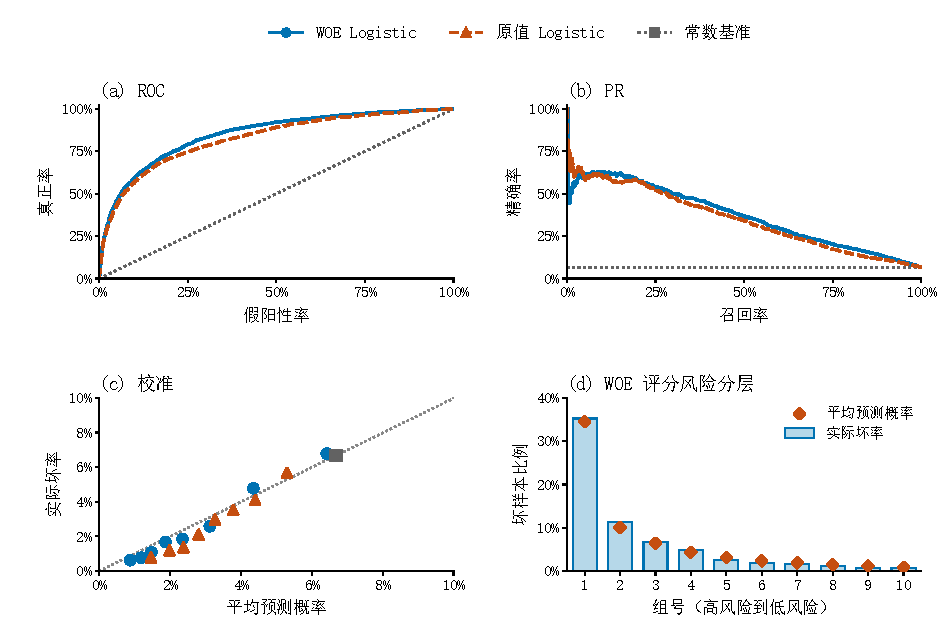
\includegraphics[width=\linewidth,trim=6bp 145bp 1bp 3bp,clip]{figures/test_evaluation.pdf}
  \caption{三模型的 ROC 与 PR 曲线}
  \label{fig:evaluation-roc-pr}
\end{figure}

图~\ref{fig:evaluation-roc-pr}(b) 以召回率为横轴，精确率 $\mathrm{TP}/(\mathrm{TP}+\mathrm{FP})$ 为纵轴，
展示随阈值变化的坏样本覆盖程度与标记对象中坏样本的占比。
记阈值由高到低变化时的召回率与精确率为 $R_j,P_j$，则
$\mathrm{AP}=\sum_j(R_j-R_{j-1})P_j$，按新增召回量加权，召回量不变的点权重为零。
WOE 模型的 AP 为 0.3681，原值模型为 0.3484，常数基准的 AP 等于测试坏样本率 0.0668。
WOE 模型的 AP 约为该基准的 5.51 倍。图中的 PR 水平虚线即测试坏样本率。

测试集坏样本仅占 6.68\%。常数基准在 $t=0.5$ 时漏掉全部坏样本（即坏样本召回率为0漏掉全部坏样本），准确率仍有 93.32\%。
沿图~\ref{fig:evaluation-roc-pr}(b) 的 WOE 曲线从 $t=0.5$ 下调阈值，召回率由 18.15\% 升至 50.02\%，
检出由 364 条增至 1,003 条，误报由 244 条增至 1,722 条。新增误报多于新增检出，总体准确率由 93.72\% 降至 90.92\%。
精确率（precision）则从 59.87\%（364/608）降至 36.81\%（1,003/2,725）。

表~\ref{tab:evaluation-recall-example} 取两模型召回率首次达到 50\% 的曲线点。
同样检出 1,003 条坏样本时，WOE 模型少误报 219 条好样本，精确率由原值模型的 34.07\% 提高至 36.81\%。

\begin{table}[!htbp]
  \centering
  \caption{召回率约 50\% 时的坏样本检出对照}
  \label{tab:evaluation-recall-example}
  \small
  \begin{tabular}{lrrrrr}
    \toprule
    模型 & 检出坏样本 & 误报好样本 & 标记总人数 & 召回率 & 精确率 \\
    \midrule
    WOE Logistic & 1,003 & 1,722 & 2,725 & 50.02\% & 36.81\% \\
    原值 Logistic & 1,003 & 1,941 & 2,944 & 50.02\% & 34.07\% \\
    \bottomrule
  \end{tabular}
\end{table}

\FloatBarrier
下一模块将在验证集上，按误报与漏报代价选择风险标记阈值，按坏样本率上限与最低接受比例选择模拟接受门槛。
冻结后再用测试集评价，说明业务目标如何决定复核或接受范围。

\subsection{概率损失与校准表现}
令 $y_i\in\{0,1\}$ 为实际标签。Brier 分数度量概率的平方误差，对数损失会加重对自信但错误的预测的惩罚。
\[
  \mathrm{Brier}=\frac{1}{n}\sum_{i=1}^n(\widehat p_i-y_i)^2,\qquad
  \mathrm{LogLoss}=-\frac{1}{n}\sum_{i=1}^n
  \bigl[y_i\ln\widehat p_i+(1-y_i)\ln(1-\widehat p_i)\bigr].
\]

与原值模型相比，WOE 模型的 Brier 分数由 0.05226 降至 0.05073，对数损失由 0.19481 降至 0.18599，
相对下降 2.91\% 和 4.53\%。常数基准的两项损失均最高。
概率损失综合反映逐户预测误差，校准图进一步显示哪些风险组的平均预测偏高或偏低。


\begin{figure}[!htbp]
  \centering
  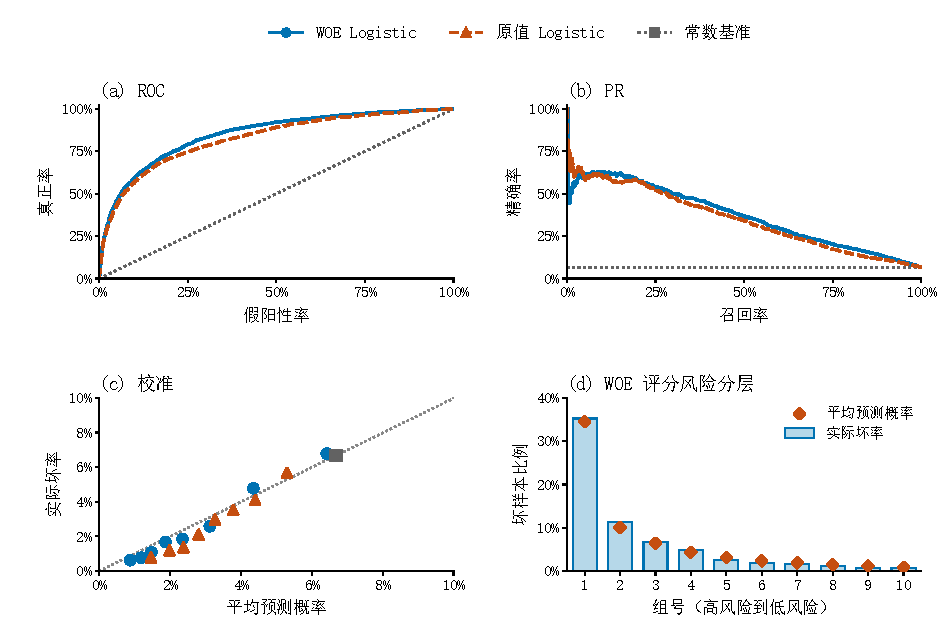
\includegraphics[width=0.66\linewidth,trim=14bp 5bp 222bp 174bp,clip]{figures/test_evaluation.pdf}
  \caption{三模型的测试集校准图（0--10\% 局部放大）}
  \label{fig:evaluation-calibration}

  \smallskip
  \parbox{0.91\linewidth}{\small 注：蓝色圆点为 WOE Logistic，橙色三角为原值 Logistic，灰色方点为常数基准。}
\end{figure}

两个 Logistic 模型分别按各自的预测风险降序分为十组，边界取最接近目标十分位的同值块末尾。
同一预测值的记录归入同组，故 WOE 各组人数介于 2,968 与 3,040，
原值模型恰好每组 3,000 人。设第 $g$ 组有 $n_g$ 人，比较平均预测概率 $\bar p_g$ 与实测坏率
$\bar y_g$。图~\ref{fig:evaluation-calibration} 的对角线表示两者相等，点在线上方表示该组风险被低估。
测试集中，WOE 和原值 Logistic 的逐户预测概率不超过 10\% 的比例分别为 85.77\% 和 87.87\%，
因此图中两轴均放大至 0--10\%。两个模型各有八组的平均预测概率和实际坏率同时落在该区间。
表~\ref{tab:evaluation-calibration} 列出每组人数和偏差，两模型的同序号组各自按预测风险划分。

\begin{table}[H]
  \centering
  \caption{两个 Logistic 模型的分组校准明细}
  \label{tab:evaluation-calibration}
  \small
  \begin{tabular}{c rrrr rrrr}
\toprule
& \multicolumn{4}{c}{WOE Logistic} & \multicolumn{4}{c}{原值 Logistic} \\
\cmidrule(lr){2-5}\cmidrule(lr){6-9}
组 & 人数 & 平均预测 & 实际坏率 & 差值 & 人数 & 平均预测 & 实际坏率 & 差值 \\
\midrule
1 & 3,001 & 34.50\% & 35.25\% & $+0.75$ & 3,000 & 32.48\% & 33.80\% & $+1.32$ \\
2 & 3,010 & 10.07\% & 11.43\% & $+1.36$ & 3,000 & 8.33\% & 11.33\% & $+3.01$ \\
3 & 2,992 & 6.42\% & 6.78\% & $+0.36$ & 3,000 & 5.30\% & 5.67\% & $+0.37$ \\
4 & 2,992 & 4.35\% & 4.78\% & $+0.43$ & 3,000 & 4.40\% & 4.10\% & $-0.30$ \\
5 & 2,980 & 3.12\% & 2.58\% & $-0.54$ & 3,000 & 3.78\% & 3.53\% & $-0.25$ \\
6 & 3,029 & 2.35\% & 1.85\% & $-0.50$ & 3,000 & 3.27\% & 2.97\% & $-0.30$ \\
7 & 2,992 & 1.87\% & 1.67\% & $-0.20$ & 3,000 & 2.81\% & 2.10\% & $-0.71$ \\
8 & 2,968 & 1.47\% & 1.08\% & $-0.40$ & 3,000 & 2.38\% & 1.37\% & $-1.01$ \\
9 & 2,996 & 1.19\% & 0.77\% & $-0.42$ & 3,000 & 1.98\% & 1.20\% & $-0.78$ \\
10 & 3,040 & 0.88\% & 0.62\% & $-0.25$ & 3,000 & 1.46\% & 0.77\% & $-0.70$ \\
\bottomrule
\end{tabular}


  \smallskip
  \parbox{0.94\linewidth}{\small 注：差值为实际坏率减平均预测概率，单位为百分点。常数基准单列一组，共 30,000 人，平均预测为 6.6844\%，实际坏率为 6.6833\%。}
\end{table}

WOE 模型前四组的平均预测低于实际坏率，后六组则偏高。偏差最明显的是第 2 组，
预测为 10.07\%，实际为 11.43\%。原值模型同序号组的预测为 8.33\%，
实际为 11.33\%。按人数加权的绝对组差
$\sum_g(n_g/n)|\bar y_g-\bar p_g|$ 在 WOE 模型为 0.52\%，在原值模型为 0.87\%。
这一统计量依赖分组方式。


\subsection{WOE 评分的风险分层}
按式~\eqref{eq:score-probability}，未取整总分越低，预测坏样本概率越高。
将测试记录按未取整分数升序排列，沿用上述近似等频方法划分十组，保留每个同分块的完整性。
第 1 组是最低分、最高风险组。表~\ref{tab:evaluation-risk-groups} 列出各组观测分数范围、人数、
坏样本数、平均预测和实际坏率。第 $g$ 组的累计覆盖率为前 $g$ 组坏样本数之和除以全部 2,005 条坏样本。

\begin{table}[H]
  \centering
  \caption{WOE 评分的十组风险分层}
  \label{tab:evaluation-risk-groups}
  \small
  \setlength{\tabcolsep}{6pt}
  \begin{tabular}{rrrrrrr}
\toprule
组 & 观测分数范围 & 人数 & 坏样本 & 平均预测 & 实际坏率 & 累计覆盖 \\
\midrule
1 & 434.095--566.542 & 3,001 & 1,058 & 34.50\% & 35.25\% & 52.77\% \\
2 & 566.579--585.813 & 3,010 & 344 & 10.07\% & 11.43\% & 69.93\% \\
3 & 585.815--598.843 & 2,992 & 203 & 6.42\% & 6.78\% & 80.05\% \\
4 & 598.849--610.015 & 2,992 & 143 & 4.35\% & 4.78\% & 87.18\% \\
5 & 610.102--618.179 & 2,980 & 77 & 3.12\% & 2.58\% & 91.02\% \\
6 & 618.193--626.538 & 3,029 & 56 & 2.35\% & 1.85\% & 93.82\% \\
7 & 626.591--632.496 & 2,992 & 50 & 1.87\% & 1.67\% & 96.31\% \\
8 & 632.615--639.667 & 2,968 & 32 & 1.47\% & 1.08\% & 97.91\% \\
9 & 639.830--647.650 & 2,996 & 23 & 1.19\% & 0.77\% & 99.05\% \\
10 & 647.982--663.133 & 3,040 & 19 & 0.88\% & 0.62\% & 100.00\% \\
\bottomrule
\end{tabular}


  \smallskip
  \parbox{0.94\linewidth}{\small 注：分数范围为本组样本的实际最小值至最大值，按三位小数展示。组别由高风险排至低风险。}
\end{table}

\begin{figure}[H]
  \centering
  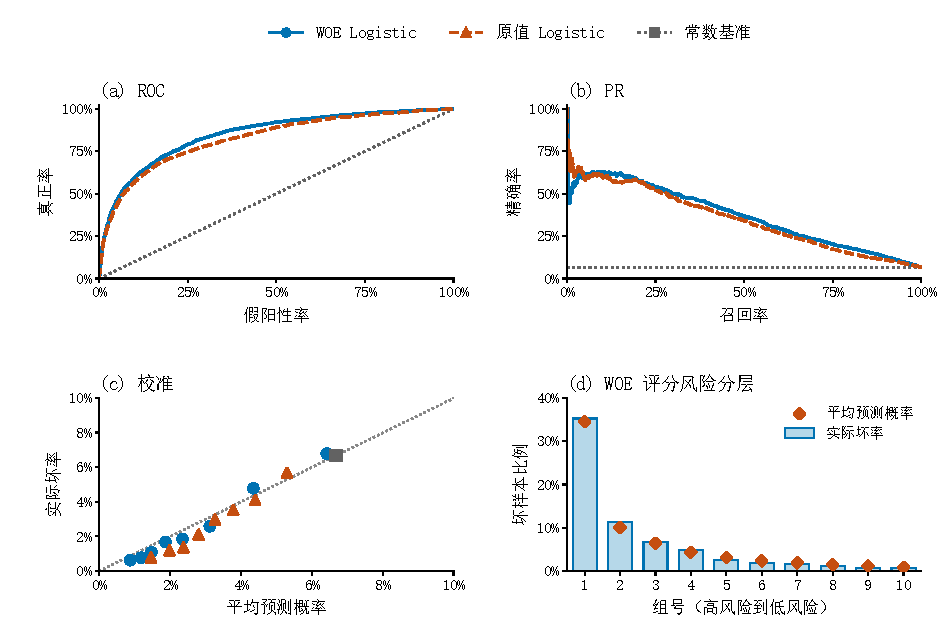
\includegraphics[width=0.66\linewidth,trim=238bp 5bp 4bp 174bp,clip]{figures/test_evaluation.pdf}
  \caption{WOE 评分各组的平均预测与实际坏率}
  \label{fig:evaluation-risk-groups}
\end{figure}

图~\ref{fig:evaluation-risk-groups} 显示，实际坏率随分数提高逐组下降。
第 1 组坏率为 35.25\%，约为总体坏率的 5.28 倍。第 2 组降至 11.43\%，第 3 组为 6.78\%，接近总体水平。
最低风险组 3,040 人中有 19 条坏样本，坏率为 0.625\%。这一结果表明评分在测试集中形成了可观察的风险梯度。

按风险从高到低检查客户时，先覆盖第 1 组约 10.00\% 的记录，就能覆盖 1,058 条坏样本，
占全部坏样本的 52.77\%。覆盖前两组约 20.04\% 的记录时，累计覆盖率提高到 69.93\%。
再纳入第 3 组，覆盖 9,003 人（30.01\%）和 1,605 条坏样本（80.05\%）。
边际检出率随检查范围扩大而降低，例如第 3 组每百人约检出 7 条坏样本，低于第 1 组的约 35 条。
这些比例描述测试集上的风险集中程度，供后续分析处理容量与检出量的取舍。


\Needspace{9\baselineskip}
\section{阈值选择与业务决策}
\label{sec:decision-thresholds}
% !TeX root = ../main.tex
本节用冻结的 WOE Logistic 概率和未取整评分，在验证集选定规则后，以同一批
30,000 条测试记录评价。误报和漏报成本、审批坏率目标均为教学情景设定。

\subsection{代价敏感的风险标记}
设客户的坏样本概率为 $p$。标记好客户产生误报成本 $C_{\mathrm{FP}}=1$，
放过坏客户产生漏报成本 $C_{\mathrm{FN}}=5$。在概率可信且成本适用于每位客户时，
标记的条件期望成本为 $1-p$，放过的条件期望成本为 $5p$。取等号时标记，得到
\[
  1-p\leq 5p \quad\Longleftrightarrow\quad
  p\geq t_{\mathrm{theory}}=\frac{1}{1+5}=\frac16 .
\]
以冻结模型的预测概率 $\widehat p$ 执行时，由式~\eqref{eq:score-probability} 得到等价分数规则
\[
  \widehat p\geq t\quad\Longleftrightarrow\quad
  S\leq s(t),\qquad s(t)=A+B\ln\frac{1-t}{t}.
\]

验证前固定概率网格 $0.01,0.02,\ldots,0.99$，另纳入 $1/6$。以
$(\mathrm{FP}+5\,\mathrm{FN})/n$ 最小为准，同成本时取较高阈值以减少标记量。
验证集最优阈值为 $0.13$，均成本为 $0.21060$，对应 $S\leq 569.891525\ldots$。
同一验证集上，$0.5$ 和 $1/6$ 的均成本分别为 $0.28133$ 和 $0.21730$。
冻结 $0.13$ 后，按表~\ref{tab:decision-flag-results} 在测试集比较三种规则。

\begin{table}[H]
  \centering
  \caption{三种风险标记规则的测试集比较}
  \label{tab:decision-flag-results}
  \small
  \setlength{\tabcolsep}{3.5pt}
  \begin{tabular}{lrrrrrrrrr}
\toprule
规则 & 分数上限 & TN & FP & FN & TP & 标记率 & 召回率 & 精确率 & 均成本 \\
\midrule
基准 0.5 & 515.041 & 27,751 & 244 & 1,641 & 364 & 2.03\% & 18.15\% & 59.87\% & 0.28163 \\
理论 $1/6$ & 561.480 & 26,434 & 1,561 & 1,041 & 964 & 8.42\% & 48.08\% & 38.18\% & 0.22553 \\
验证 0.13 & 569.892 & 25,830 & 2,165 & 905 & 1,100 & 10.88\% & 54.86\% & 33.69\% & 0.22300 \\
\bottomrule
\end{tabular}


  \smallskip
\end{table}

表~\ref{tab:decision-confusion-matrices} 按实际类别展开三种规则的混淆矩阵。坏样本为正类，
好样本行中的标记人数为误报（FP），坏样本行中的未标记人数为漏报（FN）。

\begin{table}[H]
  \centering
  \caption{三种风险标记规则的测试集混淆矩阵}
  \label{tab:decision-confusion-matrices}
  \small
  \begin{tabular}{lrrrrrr}
    \toprule
    & \multicolumn{2}{c}{基准 \(t=0.5\)}
    & \multicolumn{2}{c}{理论 \(t=1/6\)}
    & \multicolumn{2}{c}{验证选定 \(t=0.13\)} \\
    \cmidrule(lr){2-3}\cmidrule(lr){4-5}\cmidrule(lr){6-7}
    实际类别 & 未标记 & 标记 & 未标记 & 标记 & 未标记 & 标记 \\
    \midrule
    好样本 & 27,751 & 244 & 26,434 & 1,561 & 25,830 & 2,165 \\
    坏样本 & 1,641 & 364 & 1,041 & 964 & 905 & 1,100 \\
    \bottomrule
  \end{tabular}
\end{table}

$0.5$ 只标记 608 户，精确率为 59.87\%，但漏掉 1,641 条坏样本，均成本最高。
由 $1/6$ 降至 $0.13$ 后，标记量由 2,525 户增至 3,265 户，少漏 136 条坏样本，多误报 604 户。
少漏带来的成本节省为 $136\times5=680$，扣除新增误报成本后净省 76，均成本由 0.22553 降至 0.22300。
验证阈值在三种规则中成本最低，同时需要处理测试集约 10.88\% 的客户，精确率降至 33.69\%。

\Needspace{23\baselineskip}
\subsection{坏率约束下的模拟审批}
给定整数分数门槛 $c$，接受所有未取整评分 $S_i\geq c$ 的客户，同分者使用同一规则。
设验证集接受人数为 $N_c$、其中坏样本数为 $D_c$、验证集总人数为 $n_{\mathrm{val}}$。
在事先固定的 $c=300,301,\ldots,900$ 上求
\[
  \max_c\ \frac{N_c}{n_{\mathrm{val}}}
  \qquad\text{满足}\qquad
  \frac{D_c}{N_c}\leq 5\%,\qquad
  \frac{N_c}{n_{\mathrm{val}}}\geq 10\%.
\]

同接受人数时取较高门槛，若无可行门槛则报告不可行。
验证集在 530 分时接受 28,973 户，坏率为 5.03\%，超出约束。
遍历网格后，531 分是可行门槛中接受人数最多的方案，接受 28,928 户，坏率为 4.97\%。
测试阶段沿用这一门槛，结果见表~\ref{tab:decision-approval-results}。

\begin{table}[H]
  \centering
  \caption{冻结审批门槛在验证集与测试集上的表现}
  \label{tab:decision-approval-results}
  \small
  \setlength{\tabcolsep}{5pt}
  \begin{tabular}{lrrrrrrr}
\toprule
样本 & 门槛 & 接受人数 & 接受率 & 坏样本 & 平均预测 & 实际坏率 & 95\% 区间 \\
\midrule
验证集 & 531 & 28,928 & 96.43\% & 1,437 & 4.72\% & 4.97\% & -- \\
测试集 & 531 & 28,974 & 96.58\% & 1,465 & 4.79\% & 5.06\% & ［4.81\%, 5.31\%］ \\
\bottomrule
\end{tabular}


  \smallskip
  \parbox{0.96\linewidth}{\small 区间为测试集接受样本实际坏率的记录层面 Wilson 95\% 二项比例区间。}
\end{table}

测试集接受率为 96.58\%，接受者平均预测为 4.79\%，实际坏率为 5.06\%。
点估计超过 5\% 目标约 0.06 个百分点，区间 $[4.81\%,5.31\%]$ 跨越 5\%。
据此记录测试点估计超标，保留冻结门槛 531 分。区间表明，接受者坏率在 5\% 附近仍有抽样不确定性。

按本报告的评分刻度，600 分对应好坏几率 $19:1$，预测坏样本概率为 $1/(19+1)=5\%$。
对一位恰好得 600 分的客户，这表示模型根据评分时已知的信息，估计其未来两年内发生严重逾期或更严重情形的概率为 5\%。
若规定 $S\geq 600$ 时接受，每位接受者的预测概率都不超过 5\%，客群的平均预测概率也不超过 5\%。
实际坏样本率则要等两年表现窗口结束后，用发生目标事件的人数除以接受人数计算。
受模型校准偏差和样本波动影响，实际坏样本率可能超过 5\%。本方案约束的是验证集的客群实际坏样本率，
因此允许部分预测概率高于 5\% 的客户被接受。

\paragraph{两种规则的行动目标}
风险标记用于安排复核，在给定误报和漏报代价下比较标记量、检出量与成本。
模拟审批则在客群坏率约束下扩大接受范围。例如，未取整分数在 $531$ 到 $569.891525\ldots$ 之间的客户，
可同时满足接受与风险标记条件。现有数据支持比较复核容量和模拟接受风险。
若要评价实际授信收益或优化审批政策，还需结合贷款收益、违约损失率与拒绝样本的后续表现。


\Needspace{15\baselineskip}
\section{选做拓展：评分分布的 PSI}
\label{sec:score-psi}
% !TeX root = ../main.tex
\paragraph{冻结分数档}
以 90,000 条训练记录的 WOE 未取整总分为基准，在完整同分块之间选择最接近训练十分位的位置切分。
每档右端取该档训练样本的最大分数，等于切点的记录归较低一档，两端使用开口区间。
切点保存后，将同一套分档原样应用于 30,000 条测试记录。

\paragraph{计算口径}
令 $p_k$ 和 $q_k$ 分别为训练集和测试集落入第 $k$ 档的比例，评分分布的群体稳定性指标为
\[
  \mathrm{PSI}=\sum_{k=1}^{K}(q_k-p_k)\ln\frac{q_k}{p_k}.
\]
若任一档在任一子集中人数为零，则两个子集的每一档均加 $0.5$，
再分别以各自总人数加 $0.5K$ 归一化，避免零比例进入对数。
表~\ref{tab:score-psi} 中每档均有记录，本次直接使用实际占比。

\begin{table}[H]
  \centering
  \caption{训练集与测试集的固定分数档占比及 PSI}
  \label{tab:score-psi}
  \small
  \setlength{\tabcolsep}{5pt}
  \begin{tabular}{rlrrrrr}
\toprule
档 & 未取整分数范围 & 训练人数 & 训练比例 & 测试人数 & 测试比例 & PSI 分项 \\
\midrule
1 & $(-\infty, 565.795]$ & 8,999 & 10.00\% & 2,956 & 9.85\% & 0.000021 \\
2 & $(565.795, 584.817]$ & 8,992 & 9.99\% & 2,922 & 9.74\% & 0.000064 \\
3 & $(584.817, 598.843]$ & 9,065 & 10.07\% & 3,125 & 10.42\% & 0.000116 \\
4 & $(598.843, 610.102]$ & 8,996 & 10.00\% & 3,033 & 10.11\% & 0.000013 \\
5 & $(610.102, 618.406]$ & 8,964 & 9.96\% & 3,044 & 10.15\% & 0.000035 \\
6 & $(618.406, 626.591]$ & 8,985 & 9.98\% & 2,926 & 9.75\% & 0.000054 \\
7 & $(626.591, 633.237]$ & 8,984 & 9.98\% & 3,070 & 10.23\% & 0.000062 \\
8 & $(633.237, 639.830]$ & 9,204 & 10.23\% & 3,065 & 10.22\% & 0.000000 \\
9 & $(639.830, 647.650]$ & 8,657 & 9.62\% & 2,819 & 9.40\% & 0.000052 \\
10 & $(647.650, +\infty)$ & 9,154 & 10.17\% & 3,040 & 10.13\% & 0.000001 \\
\midrule
 & 合计 & 90,000 & 100.00\% & 30,000 & 100.00\% & 0.000418 \\
\bottomrule
\end{tabular}

  \smallskip

  \parbox{0.95\linewidth}{\small 切点按三位小数展示，分档使用完整精度。PSI 合计按未舍入的各档分项求和。}
\end{table}

\paragraph{结果解释}
总 PSI 为 $0.000418$。贡献最大的第 3 档，训练和测试占比分别为 $10.07\%$ 和 $10.42\%$，
按原始比例计算相差约 $0.34\%$ 。整体来看，两个随机子集在固定分数档上的分布接近。
由于样本来自同一数据集的分层随机划分，这一比较反映的是随机留出样本之间的分布差异。
检验跨期稳定性需要按评分日期获取后续客群，并沿用同一模型和固定分数档作比较。


\Needspace{24\baselineskip}
\appendix
\section{模块与 Python 复现文件}
\label{app:python-files}
% !TeX root = ../main.tex
表~\ref{tab:python-files} 按报告模块列出运行入口。脚本沿用项目目录结构，
在仓库根目录运行 \path{python run_pipeline.py} 可复现数值结果。表中列出各阶段的独立入口。

\begin{table}[H]
  \centering
  \caption{报告模块与 Python 文件对照}
  \label{tab:python-files}
  \small
  \renewcommand{\arraystretch}{1.2}
  \begin{tabular}{@{}p{0.34\linewidth}p{0.60\linewidth}@{}}
    \toprule
    开发环节 & 对应文件 \\
    \midrule
    模块一　样本划分与重复检查 & \path{scripts/split_samples.py} \\
    模块二　审计、风险分析与清洗 &
      \path{scripts/audit_data.py}、\path{scripts/feature_risk.py}\newline
      \path{scripts/preprocess.py} \\
    模块三　分箱、WOE 与 IV & \path{scripts/binning_woe.py} \\
    模块四　Logistic 与基准比较 & \path{scripts/fit_logistic.py} \\
    模块五　评分卡与逐户核验 & \path{scripts/scorecard.py} \\
    模块六　模型评价与风险分层 & \path{scripts/evaluate_models.py} \\
    模块七　阈值选择与业务决策 & \path{scripts/decision_thresholds.py} \\
    选做拓展　评分分布 PSI & \path{scripts/score_psi.py} \\
    公共依赖　绘图与检查 &
      \path{utils/setup_style.py}、\path{utils/plot_style.py}\newline
      \path{utils/export_figure.py}、\path{utils/visual_qa.py} \\
    \bottomrule
  \end{tabular}
\end{table}

\paragraph{输入与运行顺序}
将 Kaggle 原始 \path{cs-training.csv} 与 \mbox{\texttt{Data Dictionary.xls}} 放在项目根目录。
样本划分种子为 \texttt{20261103}。模块七先用参数 \texttt{freeze} 在验证集上冻结阈值，
再用 \texttt{evaluate} 评价测试集。程序将结果写入 \path{results/}，图形写入 \path{figures/}。

\paragraph{Python 环境}
Python 3.12。主要依赖为 NumPy 2.3.4、pandas 2.3.3、SciPy 1.16.2、scikit-learn 1.7.2、
Matplotlib 3.10.7、Pillow 12.0.0、PyMuPDF 1.28.2、xlrd 2.0.2。


\end{document}
